% This is "sig-alternate.tex" V1.9 April 2009
% This file should be compiled with V2.4 of "sig-alternate.cls" April 2009
%
% This example file demonstrates the use of the 'sig-alternate.cls'
% V2.4 LaTeX2e document class file. It is for those submitting
% articles to ACM Conference Proceedings WHO DO NOT WISH TO
% STRICTLY ADHERE TO THE SIGS (PUBS-BOARD-ENDORSED) STYLE.
% The 'sig-alternate.cls' file will produce a similar-looking,
% albeit, 'tighter' paper resulting in, invariably, fewer pages.
%
% ----------------------------------------------------------------------------------------------------------------
% This .tex file (and associated .cls V2.4) produces:
%       1) The Permission Statement
%       2) The Conference (location) Info information
%       3) The Copyright Line with ACM data
%       4) NO page numbers
%
% as against the acm_proc_article-sp.cls file which
% DOES NOT produce 1) thru' 3) above.
%
% Using 'sig-alternate.cls' you have control, however, from within
% the source .tex file, over both the CopyrightYear
% (defaulted to 200X) and the ACM Copyright Data
% (defaulted to X-XXXXX-XX-X/XX/XX).
% e.g.
% \CopyrightYear{2007} will cause 2007 to appear in the copyright line.
% \crdata{0-12345-67-8/90/12} will cause 0-12345-67-8/90/12 to appear in the copyright line.
%
% ---------------------------------------------------------------------------------------------------------------
% This .tex source is an example which *does* use
% the .bib file (from which the .bbl file % is produced).
% REMEMBER HOWEVER: After having produced the .bbl file,
% and prior to final submission, you *NEED* to 'insert'
% your .bbl file into your source .tex file so as to provide
% ONE 'self-contained' source file.
%
% ================= IF YOU HAVE QUESTIONS =======================
% Questions regarding the SIGS styles, SIGS policies and
% procedures, Conferences etc. should be sent to
% Adrienne Griscti (griscti@acm.org)
%
% Technical questions _only_ to
% Gerald Murray (murray@hq.acm.org)
% ===============================================================
%
% For tracking purposes - this is V1.9 - April 2009

\documentclass{sig-alternate}
  \pdfpagewidth=8.5truein
  \pdfpageheight=11truein

% Remove copyright space
\makeatletter
\def\@copyrightspace{\relax}
\makeatother

% Packages
\usepackage[table,xcdraw]{xcolor}
\usepackage{hyperref}
\usepackage{enumitem}
\usepackage{booktabs,caption}
\usepackage{tabularx}
\usepackage[flushleft]{threeparttable}

% Creating a custom itemize
\setlistdepth{5}

\newlist{longitem}{itemize}{5}
\setlist[longitem,1]{label={--}}
\setlist[longitem,2]{label={--}}
\setlist[longitem,3]{label={--}}
\setlist[longitem,4]{label={--}}
\setlist[longitem,5]{label={--}}

% Custom column type for tabularx environment. Centers and fills
\newcolumntype{Y}{>{\centering\arraybackslash}X}

\begin{document}

\title{Detecting emotion with a pressure sensitive touchscreen}
\subtitle{[...]}


\numberofauthors{1} %  in this sample file, there are a *total*
% of EIGHT authors. SIX appear on the 'first-page' (for formatting
% reasons) and the remaining two appear in the \additionalauthors section.
%
\author{
% You can go ahead and credit any number of authors here,
% e.g. one 'row of three' or two rows (consisting of one row of three
% and a second row of one, two or three).
%{}
% The command \alignauthor (no curly braces needed) should	
% precede each author name, affiliation/snail-mail address and
% e-mail address. Additionally, tag each line of
% affiliation/address with \affaddr, and tag the
% e-mail address with \email.
%
% 1st. author
\alignauthor Kevin Blom\\
       \affaddr{University of Amsterdam}\\
       \affaddr{Science Park 904}\\
       \email{xxxxxx@xxxxxx.xx}
}

\maketitle

\begin{abstract}
	
\end{abstract}

\section{Introduction} % (fold)
\label{sec:introduction}
Affective computing as introduced by Picard\cite{Picard1995} in 1995 lays a foundation for computers and technology to incorporate the recognition and expression of emotions. It can provide better performance when assisting humans or enhance the computers ability to make decisions. It does not have the goal of making computers more human-like, but it is more practical in nature; make computers function with intelligence and sensitivity towards its users\cite{Picard1997}.  According to Shah et al.\cite{Shah2015} there are two general models to represent emotion; discrete and continuous. The discrete model represent emotions that are measurable and physiologically distinct like angry, sad, happy, etc. \cite{Ekman1992} The continuous model represents emotions on a two-dimensional scale, where one axis represents \textit{valence} and the other \textit{arousal} \cite{Posner2005}. Mauss et al. \cite{Mauss2009} suggest that using a dimensional framework is a better option when capturing emotion, relative to discrete frameworks. Since, the measuring of emotion has been a subject of research and several different angles have been discovered to approach it.

\subsection{Physiological detection} % (fold)
\label{sub:physiology}
One angle uses physiological signals of the human body to measure and detect emotion. In a review by Wioleta\cite{Wioleta2013}, eight studies were collected that measure emotion using one or more physiological signals combined. These signals are \textit{EEG, skin conductance, blood volume pulse, temperature, heart rate, blood pressure, respiration, EMG,} and \textit{ECG}. Most of these physiological signals have the drawback that they need specialized sensors attached to the body, making unobtrusive measurements difficult. With the recent rise of smart wearables, heart rate is one of the signals that is more readily available to use in applications on smart devices.
% subsection physiology (end)

\subsection{Facial detection} % (fold)
\label{sub:facial_detection}
Facial detection of emotion incorporates the measurement of facial muscle movement, voice or speech \cite{Ververidis2004}, and also includes the eye as point of detection, i.e. movement, blinking, and pupil dilation \cite{Soleymani2015}. By connecting facial muscle movement to visual display of emotions, Ekman et al. \cite{Ekman1969} conclude with a basic set of six mutually exclusive emotions that could be recognized. Expanding, De Silva et al. \cite{Silva1997} found that several emotions are expressed by either visual or auditory cues, or both, meaning that some emotions can be recognized by visual cues alone, auditory cues alone, or need a combination of both to be detected accurately.
% subsection facial_emotion_detection (end)

\subsection{Posture/gestures emotion detection}
Other means of detection emotions involve the tracking and interpretation of posture and gesture. Wallbott et al. \cite{Wallbott1998} concluded in 1998 that there are, in some cases, distinctive patterns of movement and postural behavior that have a strong correlation to emotions. In other cases, they mention that in absence of patterns there are still distinctive features from which emotion could be inferred. Coulson et al. \cite{Coulson2004} researched static body postures and the recognition of emotions from these body postures by participants. It showed that disgust is a tough emotion to recognize but anger and sadness had over 90\% correct detection rates. Furthermore, happiness and surprise were two emotions that were often confused. 

\subsection{Practical applications} % (fold)
\label{sub:practical_applications}
Looking at a more practical and applied side of emotion detection, Gao et al. \cite{Gao2012} used touchscreen devices, where the application of gestures on touch screens was successfully linked to emotional states with the use of a game. The emotional states that were tested for are: excited, relaxed, frustrated and bored, and accuracy of detection reached at minimum 69\%. However, the research of Gao et al. was limited to gestures and did not incorporate data from taps. Furthermore, Lv et al. \cite{H.R.LvZ.L.LinW.J.Yin2008} have created means to detect emotion from keyboard pressure using feature extraction. This indicates that the use of a keyboard on a touch screen could also be used as means of detecting emotion, but one must keep in mind that a regular keyboard is not fully comparable to a touchscreen keyboard. It lays flat on a desk, and is often typed upon with more than one or two fingers, which means that the pressure exerted on the keyboard is likely not directly correlated with the pressure on a touchscreen keyboard. Moreover, Lee et al \cite{Lee2012} propose an unobtrusive way of detecting emotion by analyzing smartphone usage patterns (not unlike LiKamWa et al. \cite{Likamwa2013}) and social network status updates. However, this required that the user would post status updates through independently developed social networking applications, that are not officially supported by the social networks themselves.

% subsection practical_applications (end)

\subsection{Research Question}
From the related work can be concluded that most types of detection of emotions are invasive, either requiring constant monitoring, possibly with sensors attached to the body, or by constant recording of audio and visual data. The touch screen is a technology a lot of people interact with every day, where they deliberately choose to participate in those interactions. Using touch screen presses as indicators for emotional state could be an unobtrusive way of detecting emotion without the need for constant monitoring. With the introduction of pressure sensitive touchscreens in recent smart devices, an interesting new sensor is added to the plethora of sensors already available. Subsequently, this leads to the following research question:\\

\textit{Can pressure sensitive touch screen devices be used to tell more about the mood of the user?}\\
% \begin{itemize}
% 	\item Description of background.
% 	\item Explanation of why research was necessary.
% 	\item Description of how research will be undertaken.
% \end{itemize}

% section Introduction (end)

\section{Methods} % (fold)
\label{sec:methods}
In order to test for the correlation between taps on a touch screen and emotion, there has to be a standardized way of eliciting different emotions. Fortunately, there exists a photo set that has been thoroughly tested for emotional response on a two dimensional scale that is called the Geneva Affective Picture Database (GAPED) \cite{Dan-glauser2011}. Utilizing the emotional responses of this photo set as a baseline, touch screen taps and their pressure can be compared to emotional response.
Participants were selected using a convience sampling process at an office. The participants varied in age, educational level, current line of work, and background.

\subsection{Emotional elicitation} % (fold)
\label{sub:emotional_elicitation}
Using a standardized photo set that has been thoroughly researched for emotional response when showed to participants, a ground truth for emotion was set. The GAPED photo set uses the continuous model of representing emotions, i.e. the two-dimensional valence and arousal model. The photo set counts 730 pictures and is divided into 6 categories: Animal, Human, Neutral, Positive, Snakes, Spiders. From each of the categories, 10 pictures were randomly selected, resulting in a set of 60 pictures used for the experiment. Each participant was presented with the same 60 pictures, but in random order.
Brown et al. \cite{Neuroscience2012} remark that 5 second exposure to pictures is often used for the International Affective Picture System photos. The GAPED photo set has been created because of two issues with the IAPS; extensive use decreases impact of the stimuli, and the limited number of pictures for specific themes. Both these issues are not exposure time related, so the choice of exposure time of the photo to the participant is 5 seconds.

% subsection emotional_elicitation (end)

\subsection{Pressure detection} % (fold)
\label{sub:pressure_detection}
Taps were detected on an Apple iPhone 6s device with a 3D touch screen running iOS 10.3.1. The pressure of taps was registered on a floating point scale from 0.0 to 6.67 (Corresponding with 0 to $\pm$350 grams) and for every tap, several pressure measurements were registered in chronological order. Furthermore, the duration of a tap was registered in order to create pressure-over-time graphs for every tap.
% subsection pressure_detection (end)

\subsection{Data collection} % (fold)
\label{sub:data_collection}
In order to collect a larger data set, 4 taps per photo were required to advance to the next photo. These taps are directed with the use of gray colored buttons that are randomly shown on a 4 by 4 grid on the screen (Figure \ref{fig:grid}). The random pattern of the buttons ensures that the position of the tap on the screen does not matter for the pressure measurement. The gray color is used because it is perceived as neutral. The buttons are random for every photo, and for every participant. In other words, no participant received the same grid for the same photo.
\begin{figure}[h]
    \centering
    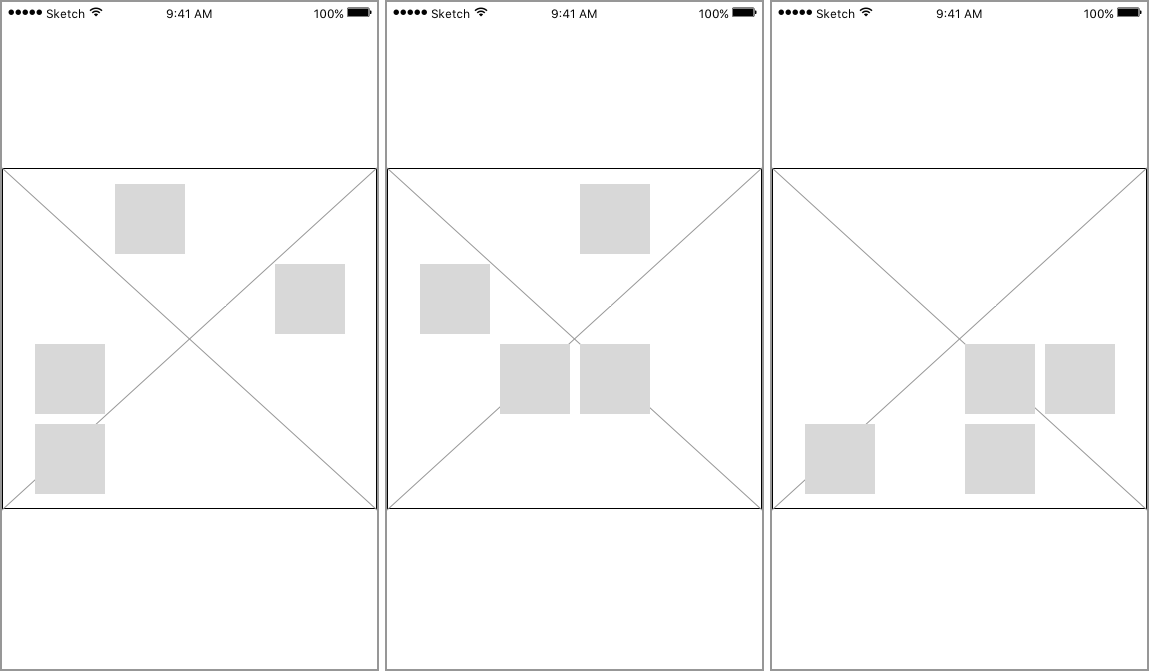
\includegraphics[width=0.5\textwidth]{images/Grid.png}
    \caption{Three examples of the grid as presented over a picture.}
    \label{fig:grid}
\end{figure}

All the data that was collected was anonymously and securely sent realtime to a Firebase\footnote{\url{http://firebase.google.com/}} database. Firebase utilizes a JSON\footnote{\url{http://www.json.org}} tree structure that can be described as in Figure \ref{fig:datastructure}.
% \begin{figure}[h]
%     \centering
%     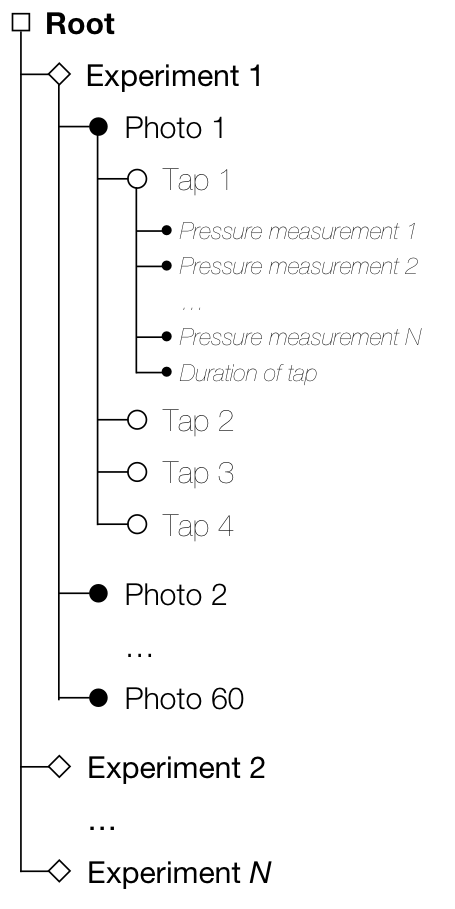
\includegraphics[width=0.3\textwidth]{images/Datastructure.png}
%     \caption{Database structure in simplified form.}
%     \label{fig:datastructure}
% \end{figure}

% subsection data_collection (end)

\subsection{Experiment setup} % (fold)
\label{sub:experiment_setup}
Firstly, participants were told what the expirement entailed and were presented with a consent form. Subsequently, the participants continued the experiment on the smart device with test application. The test application is structured as follows:
\begin{enumerate}
	\item Participant is presented with a screen that asks if they received and signed a consent form and if not, that they should contact the supervisor immediately. There is also a \textit{start} button to start the experiment.
	\item The participant is shown a picture.
	\item After 5 seconds, 4 gray buttons are shown, overlaid on the picture in a random pattern (Figure \ref{fig:grid}).
	\item When the participant pressed all the 4 buttons, the next picture is presented.
	\item This process repeats untill al 60 pictures have been shown.
	\item The participant is presented with a conclusive screen that has a thank you message and refers to the supervisor if there are questions.
\end{enumerate}
% subsection experiment_setup (end)

\subsection{Data analysis}
The collected data was interpreted in several ways.

\subsubsection{Maximum tap pressure}
The first interpretation regards maximum tap pressure. For every tap, only the maximum pressure value was extracted and subsequently averaged for every photo. This resulted in two independent variables (valence, arousal) and one dependent  variable (average maximum tap force) per photo. A multiple regression was run to predict tap pressure from valence and arousal. 

What statistical methods were used, based on what principles and data..

\begin{itemize}
	\item Overview of the research.
	\item Report of who took part and where.
	\item Report of what procedures were used.
	\item Report of what materials were used.
	\item Report of any statistical analysis used.
\end{itemize}

% section methods (end)

\section{Results} % (fold)
\label{sec:results}
\begin{itemize}
	\item Report of findings.
	\item Reference to any diagrams used.
\end{itemize}

\subsection{Maximum tap pressure}
There was linearity as assessed by partial regression plots and a plot of studentized residuals against the predicted values. There was independence of residuals, as assessed by a Durbin-Watson statistic of 1.718. There was homoscedasticity, as assessed by visual inspection of a plot of studentized residuals versus unstandardized predicted values. There was no evidence of multicollinearity, as assessed by tolerance values greater than 0.1. There were no studentized deleted residuals greater than $\pm$3 standard deviations, no leverage values greater than 0.2, and values for Cook's distance above 1. The assumption of normality was met, as assessed by Q-Q Plot. The multiple regression model did not statistically significantly predicted tap pressure, $F(2, 57) = 2.033$, $p > 0.05$, adj. $R^2$ = 0.034. Non of the variables added statistically significantly to the prediction(i.e. $p > 0.05$), with $p_{valence} = 0.35$ and $p_{arousal} = 0.079$. Regression coefficients and standard errors can be found in Table \ref{tab:summary_multiple_regression_max_pressure_avg}.

\begin{table}[ht]
\centering
	\begin{threeparttable}
		\caption{Summary of multiple regression analysis for maximum pressure average.\label{tab:summary_multiple_regression_max_pressure_avg}}
		\begin{tabularx}{0.9\linewidth}{@{}lYYY@{}}
			\toprule
			Variable  & \textit{B} & \textit{$SE_{B}$} & \textit{$\beta$} \\ \midrule
			Intercept & .375       & .024              &                  \\
			Valence   & .000       & .000              & .213             \\
			Arousal   & .001       & .000              & .403             \\ \bottomrule
		\end{tabularx}
	\begin{tablenotes}
		\small
		\item Note: \textit{B} = unstandardized regression coefficient. \textit{$SE_B$} = Standard error of the coefficient. $\beta$ = standardized coefficient.
	\end{tablenotes}
	\end{threeparttable}
\end{table}
% section results (end)

\section{Discussion} % (fold)
\label{sec:discussion}
\begin{itemize}
	\item Summary of main purpose of research.
	\item Review of most important findings.
	\item Evaluation of findings.
	\item Explanation of findings.
	\item Comparison with other researchers findings.
	\item Description of implications and recommendations.
\end{itemize}


% section discussion (end)

% The following two commands are all you need in the
% initial runs of your .tex file to
% produce the bibliography for the citations in your paper.
\bibliographystyle{abbrv}
\bibliography{library,Alternative}  % sigproc.bib is the name of the Bibliography in this case
% You must have a proper ".bib" file
%  and remember to run:
% latex bibtex latex latex
% to resolve all references
%
% ACM needs 'a single self-contained file'!
%
%APPENDICES are optional
%\balancecolumns

\end{document}